\documentclass[a4paper, 10pt]{article}
\usepackage{fullpage}
\usepackage{makecell}
\usepackage{amsmath}
\usepackage{tikz}


\usetikzlibrary{positioning}
\usetikzlibrary{automata}

\hyphenation{ent-spre-chen-der hier-aus}

\title{Übung 2}
\author{Philip Magnus}
\date{\today}

\begin{document}
\maketitle
\section*{Aufgabe 1}

\begin{center} 
    \begin{tabular}{c|c|c} 
     \hline
     Ausdruck & Landau & Erklärung \\ [0.5ex] 
     \hline\hline
     $n^{4}+12n^{3}+17n$ & $O(n^{4})$ & $n^{4}$ Term wächst am stärksten und dominiert das Wachstum der Funktion\\ 
     \hline
     $n^{3}+2n^{2}log_2 n$ & $O(n^{3})$ & \makecell{(1) hieraus ergibt sich, wenn $O(n)=c \cdot g(n)$ angewendet: $c = 3 | g(n) = n^{3}$}\\
     \hline
     $n^{2}+2^{n}$ & $O(2^{n})$ & $2^{n} \ge n^{2}\ \forall\ n>4$\\
     \hline
     $\frac{13n^{4}+7n+31}{n^{4}+1}$ & $O(1)$ & \makecell{(2)}\\
     \hline
    \end{tabular}
\end{center}

\begin{align*}
(1)\ n^{3}+2n^{2}log_2 n \le n^{3}+2n^{2} \cdot n = n^{3}+2n^{3} = 3n^{3}\\
\end{align*}
\\
\begin{align*}
(2)\ 13n^{4}+7n+31 \le 13n^{4}+n^{4}+31\ \forall\ n\ge3
\\
14n^{4}+31 \le 31n^{4}+31=31(n^{4}+1)
\\
\frac{31(n^{4}+1)}{n^{4}+1}=31
\end{align*}

\section*{Aufgabe 2}

\begin{center} 
    \begin{tabular}{c|c|c} 
     \hline
     Ausdruck & Landau & Erklärung \\ [0.5ex] 
     \hline\hline
     $3n^{2}+7n+1$ & $O(n^{2})$ & $3n^{2}+7n+1 \le 3n^{2}+n^{2}+1\ \forall\ n\ge4$\\ 
     \hline
     $(n-1)(n^{3}-n^{2})$ & $O(n^{4})$ & \makecell{$(n-1)(n^{3}-n^{2})=n^{4}-n^{3}-n^{3}+n^{2}$}\\
     \hline
     $n^{2}+log_2(log_2(n))$ & $O(n^{2})$ & $log_2(log_2(n))$ wächst sehr langsam, $n^{2}$ dominiert das Wachstum\\
     \hline
    \end{tabular}
\end{center}

\section*{Aufgabe 3}

Ist korrekt, da:\\

\begin{align*}
f(n) = O(n^{3}),\ g(n)=O(n^{2})
\\
c \cdot n^{3} \cdot c \cdot n^{2} = c^{2} \cdot n^{3} \cdot n^{2}=c^{2} \cdot n^{5}
\\
\Rightarrow O(n^{5})
\end{align*}

\newpage

\section*{Aufgabe 4}

a)\\

\begin{center}
    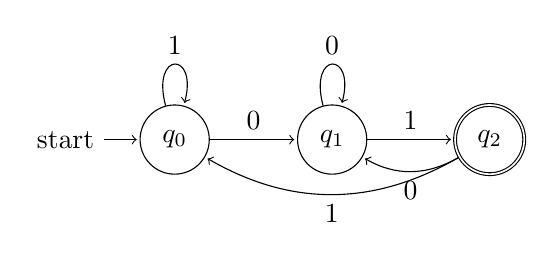
\begin{tikzpicture}[shorten >=1pt,node distance=2cm,on grid,auto]
        % \draw[help lines] (0,0) grid (3,2);

      \node[state,initial]  (q_0)                      {$q_0$};
      \node[state]          (q_1) [right=of q_0] {$q_1$};
      \node[state,accepting]          (q_2) [right=of q_1] {$q_2$};

      \path[->] (q_0) edge                         node          {0} (q_1)
                      edge [loop above]            node          {1} (q_0)
                (q_1) edge                         node          {1} (q_2)
                      edge [loop above]            node          {0} (q_2)
                (q_2) edge [bend left, below]      node          {0} (q_1)
                      edge [bend left, below]      node          {1} (q_0)
                      ;
    \end{tikzpicture}
  \end{center}

  \begin{center} 
    \begin{tabular}{c|c|c} 
     \hline
     Q & 0 & 1 \\ [0.5ex] 
     \hline\hline
     $\rightarrow q_0$ & $q_1$ & $q_0$\\ 
     \hline
     $q_1$ & $q_1$ & $q_{2}*$\\
     \hline
     $q_{2}*$ & $q_1$ & $q_0$\\
     \hline
    \end{tabular}
\end{center}

b)\\

\begin{center}
    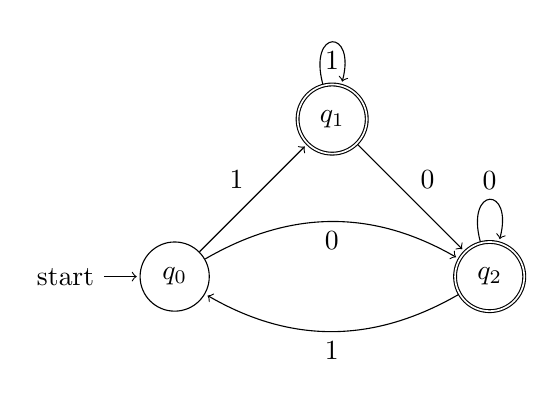
\begin{tikzpicture}[shorten >=1pt,node distance=2cm,on grid,auto]
        % \draw[help lines] (0,0) grid (3,2);

      \node[state,initial]  (q_0)                                        {$q_0$};
      \node[state, accepting, above of=q_0, right of=q_0]          (q_1) {$q_1$};
      \node[state, accepting, below of=q_1, right of=q_1]          (q_2) {$q_2$};

      \path[->] (q_0) edge                         node          {1} (q_1)
                      edge [bend left, below]      node          {0} (q_2)
                (q_1) edge                         node          {0} (q_2)
                      edge [loop above, below]     node          {1} (q_1)
                (q_2) edge [loop above]            node          {0} (q_2)
                      edge [bend left, below]      node          {1} (q_0)
                      ;
    \end{tikzpicture}
  \end{center}


\section*{Aufgabe 5}

a)\\

\begin{center}
    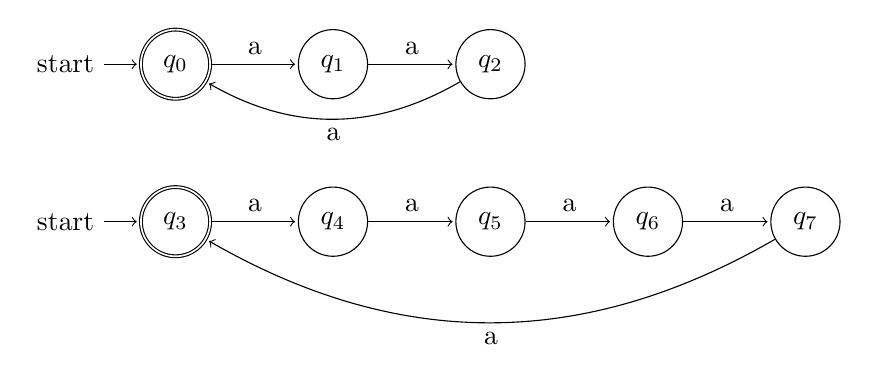
\begin{tikzpicture}[shorten >=1pt,node distance=2cm,on grid,auto]
        % \draw[help lines] (0,0) grid (3,2);

      \node[state, initial, accepting]                  (q_0) {$q_0$};
      \node[state, right of=q_0]                        (q_1) {$q_1$};
      \node[state, right of=q_1]                        (q_2) {$q_2$};
      \node[state, initial, accepting, below of=q_0]    (q_3) {$q_3$};
      \node[state, right of =q_3]                       (q_4) {$q_4$};
      \node[state, right of =q_4]                       (q_5) {$q_5$};
      \node[state, right of =q_5]                       (q_6) {$q_6$};
      \node[state, right of =q_6]                       (q_7) {$q_7$}; 

      \path[->] (q_0) edge                        node          {a} (q_1)
                (q_1) edge                        node          {a} (q_2)
                (q_2) edge [bend left, below]     node          {a} (q_0)
                (q_3) edge                        node          {a} (q_4)
                (q_4) edge                        node          {a} (q_5)
                (q_5) edge                        node          {a} (q_6)
                (q_6) edge                        node          {a} (q_7)
                (q_7) edge [bend left, below]     node          {a} (q_3)
                      ;
    \end{tikzpicture}
  \end{center}

  \newpage

  b)\\

  \begin{center} 
    \begin{tabular}{c|c|c} 
     \hline
     $\delta$ & a & $Q_{new}$\\ [0.5ex] 
     \hline\hline
     $\rightarrow \{q_0, q_3\}$ & $\{q_1, q_4\}$ & $s_{0}*$\\
     \hline
     $\{q_1, q_4\}$ & $\{q_2, q_5\}$ & $s_{1}$\\
     \hline
     $\{q_2, q_5\}$ & $\{q_0, q_6\}$ & $s_{2}$\\
     \hline
     $\{q_0, q_6\}$ & $\{q_1, q_7\}$ & $s_{3}*$\\
     \hline
     $\{q_1, q_7\}$ & $\{q_2, q_3\}$ & $s_{4}$\\
     \hline
     $\{q_2, q_3\}$ & $\{q_0, q_4\}$ & $s_{5}*$\\
     \hline
     $\{q_0, q_4\}$ & $\{q_1, q_5\}$ & $s_{6}$\\
     \hline
     $\{q_1, q_5\}$ & $\{q_2, q_6\}$ & $s_{7}$\\
     \hline
     $\{q_2, q_6\}$ & $\{q_0, q_7\}$ & $s_{8}$\\
     \hline
     $\{q_0, q_7\}$ & $\{q_1, q_3\}$ & $s_{9}*$\\
     \hline
     $\{q_1, q_3\}$ & $\{q_2, q_4\}$ & $s_{10}$\\
     \hline
     $\{q_2, q_4\}$ & $\{q_0, q_5\}$ & $s_{11}$\\
     \hline
     $\{q_0, q_5\}$ & $\{q_1, q_6\}$ & $s_{12}*$\\
     \hline
     $\{q_1, q_6\}$ & $\{q_2, q_7\}$ & $s_{13}$\\
     \hline
     $\{q_2, q_7\}$ & $\{q_0, q_3\}$ & $s_{14}$\\
     \hline
    \end{tabular}
\end{center}


\begin{center}
  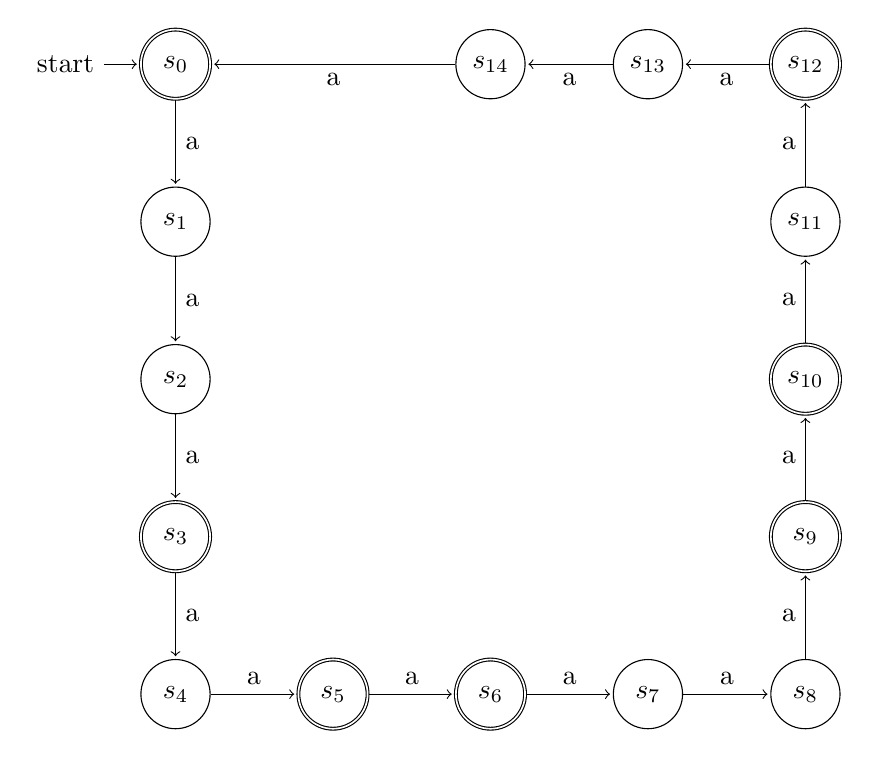
\begin{tikzpicture}[shorten >=1pt,node distance=2cm,on grid,auto]
      % \draw[help lines] (0,0) grid (3,2);

    \node[state, initial, accepting]                                            (s_0) {$s_0$};
    \node[state, below of=s_0]                                    (s_1) {$s_1$};
    \node[state, below of=s_1]                                    (s_2) {$s_2$};
    \node[state, accepting, below of=s_2]                         (s_3) {$s_3$};
    \node[state, below of=s_3]                                   (s_4) {$s_4$};
    \node[state, accepting, right of =s_4,]                        (s_5) {$s_5$};
    \node[state, accepting, right of =s_5,]                        (s_6) {$s_6$};
    \node[state, right of=s_6]                                     (s_7) {$s_7$}; 
    \node[state, right of=s_7]                                     (s_8) {$s_8$};
    \node[state, accepting, above of=s_8]                        (s_9) {$s_9$};
    \node[state, accepting, above of=s_9]                        (s_10) {$s_{10}$};
    \node[state, above of =s_10]                                  (s_11) {$s_{11}$};
    \node[state, accepting, above of =s_11]                       (s_12) {$s_{12}$};
    \node[state, left of =s_12]                                  (s_13) {$s_{13}$};
    \node[state, left of =s_13]                                  (s_14) {$s_{14}$};

    \path[->] (s_0) edge                         node          {a} (s_1)
              (s_1) edge                         node          {a} (s_2)
              (s_2) edge                         node          {a} (s_3)
              (s_3) edge                         node          {a} (s_4)
              (s_4) edge                         node          {a} (s_5)
              (s_5) edge                         node          {a} (s_6)
              (s_6) edge                         node          {a} (s_7)
              (s_7) edge                         node          {a} (s_8)
              (s_8) edge                         node          {a} (s_9)
              (s_9) edge                         node          {a} (s_10)
              (s_10) edge                        node          {a} (s_11)
              (s_11) edge                        node          {a} (s_12)
              (s_12) edge                        node          {a} (s_13)
              (s_13) edge                        node          {a} (s_14)
              (s_14) edge                        node          {a} (s_0)
                    ;
  \end{tikzpicture}
\end{center}

\newpage

\section*{Aufgabe 6}

a)\\
\\
- benötigt wird ein Zustand für OK, lesen von $0$\\
- Zustand für WARN, lesen von $1$\\
- bei lesen von $1$ aus WARN $\rightarrow$ REJCET\\
- bei lesen von Leerzeichen in Zustand WARN oder OK $\rightarrow$ ACCEPT
- bei lesen von $0$ in Zustand WARN $\rightarrow$ OK\\
\\

b)\\
\\

\begin{center} 
  \begin{tabular}{c|c|c|c|c} 
   \hline
   $Q$ & $\vdash$ & $0$ & $1$ & $\sqcup$\\ [0.5ex] 
   \hline\hline
   $OK$ & $(OK, \vdash, R)$ & $(OK, 0, R)$ & $(W, 1, R)$ & $(ACCEPT, \sqcup, R)$\\
   \hline
   $WARN$ & $-$ & $(OK, 0, R)$ & $(REJECT, 1, R)$ & $(ACCEPT, \sqcup, R)$\\
   \hline
   $ACCEPT$ & $-$ & $-$ & $-$ & $-$\\
   \hline
   $REJECTT$ & $-$ & $-$ & $-$ & $-$\\
   \hline
  \end{tabular}
\end{center}

\begin{align*}
Q=\{ OK, WARN, ACCEPT, RECJECT \}\\
\\
\Sigma=\{ 0, 1 \} \ \ \Sigma \subset \Gamma\\
\\
\Gamma=\{ 0,1,\vdash,\sqcup \}\\
\\
\delta: \ Q\times\Gamma \ \rightarrow \ Q\times\Gamma\times\{ R,L \}\\
\\
M=\{ Q, \Sigma, \Gamma, \vdash, \sqcup, \delta, OK, ACCEPT, REJECT \}\\
\end{align*}



\end{document}